\documentclass[12pt]{article}

\usepackage{graphicx}
\usepackage{paralist}
\usepackage{amsfonts}
\usepackage{amsmath}
\usepackage{hhline}
\usepackage{booktabs}
\usepackage{multirow}
\usepackage{multicol}
\usepackage{url}

\oddsidemargin -10mm
\evensidemargin -10mm
\textwidth 160mm
\textheight 200mm
\renewcommand\baselinestretch{1.0}

\pagestyle {plain}
\pagenumbering{arabic}

\newcounter{stepnum}

%% Comments

\usepackage{color}

\newif\ifcomments\commentstrue

\ifcomments
\newcommand{\authornote}[3]{\textcolor{#1}{[#3 ---#2]}}
\newcommand{\todo}[1]{\textcolor{red}{[TODO: #1]}}
\else
\newcommand{\authornote}[3]{}
\newcommand{\todo}[1]{}
\fi

\newcommand{\wss}[1]{\authornote{blue}{SS}{#1}}

\title{Assignment 4, Design Specification}
\author{SFWRENG 2AA4}

\begin{document}

\maketitle
This Module Interface Specification (MIS) document contains modules, types and
methods for implementing the game \textit{2048}. At the start of each game, the board is is randomly filled with two numbers either 2 or 4. The user has four moves in total to play the game. The keyboard keys w, a, s, d are used to move the numbers in the board along the top, left, down and right respectively. The game continues until the entire board is filled up with numbers and cannot merge anymore or if the user achieves the number 2048. The only way to win this game is to achieve 2048 in the board.

\section{Overview of the design}
This design applies Model-View-Controller (MVC) design pattern and Singleton design pattern. The MVC components are $BoardT, Movements$ (model module), $UserInterface$ (view module) and $GameController$ (controller module). Singleton design pattern is specified and implemented for $UserInterface$ and $GameController$.

\medskip

The MVC design pattern is specified and implemented in the following way: the module $BoardT$ stores the state of the game board and the status of the game. The module $Movements$ handles all the user input. A view module $UserInterface$ displays the state of the game board and game using a test-based graphics. The controller module $GameController$ is responsible for handling input actions. The design allows the board size to be anything greater than 3.


\medskip
For \textit{GameController} and \textit{UserInterface}, use the getInstance() method to obtain the abstract object.

\bigskip

\noindent A UML diagram is provided below for visualizing the structure of this software architecture.

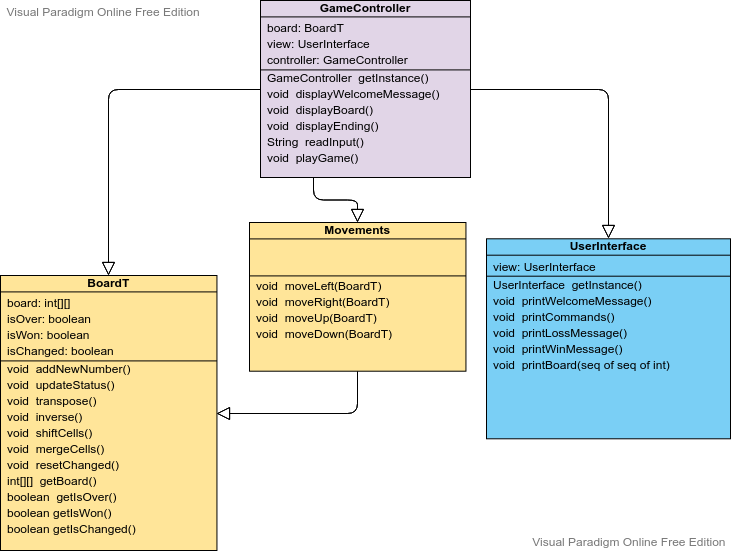
\includegraphics[width=0.9\textwidth]{MVC-UML.png}

\subsection*{Likely Changes my design considers:}
\begin{itemize}
    \item Data structure used for storing the game board.
    \item Change in the size of the game board.
    \item Change in peripheral devices for taking user input.
    \item The way the game is visually represented.
\end{itemize}

\newpage

\section* {Board ADT Module}

\subsection*{Template Module}

BoardT

\subsection* {Uses}
None
\subsection* {Syntax}
\subsubsection* {Exported Types}
BoardT = ?
\subsubsection* {Exported Constant}
None
\subsubsection* {Exported Access Programs}

\begin{tabular}{| l | l | l | l |}
\hline
\textbf{Routine name} & \textbf{In} & \textbf{Out} & \textbf{Exceptions}\\
\hline
BoardT & $\mathbb{N}$ & BoardT & IllegalArgumentException\\
\hline
addNewNumber &  &  & \\
\hline
updateStatus &  &  & \\
\hline
transpose &  &  & \\
\hline
inverse &  &  & \\
\hline
shiftCells &  &  & \\
\hline
resetChanged  &  &  & \\
\hline
getBoard  &  & seq of (seq of $\mathbb{N}$) & \\
\hline
getIsOver  &  & $\mathbb{B}$ & \\
\hline
getIsWon  &  & $\mathbb{B}$ & \\
\hline
getIsChanged   &  & $\mathbb{B}$ & \\
\hline
\end{tabular}

\subsubsection* {State Variables}

board: seq of (seq of $\mathbb{N}$) \\
isOver: $\mathbb{B}$ \\
isWon: $\mathbb{B}$ \\
changed: $\mathbb{B}$

\subsubsection* {State Invariant}
None

\subsubsection* {Assumptions}
\begin{itemize}
  \item Assume there is a random function that generates a random value between 0 and 1.
  \item Access routine addNewNumber is called two times after constructor is called.
\end{itemize}

\subsubsection* {Access Routine Semantics}

new BoardT(size):
\begin{itemize}
    \item transition: board, isOver, changed $:=$ sequence [size, size] of $\mathbb{N}$, false, false
    \item output: $out := \mathit{self}$
    \item exception: exc $:= (size < 4 \Rightarrow IllegalArgumentException)$
\end{itemize}

\noindent addNewNumber():
\begin{itemize}
    \item transition: board $:=$ Adds a number (either 2 or 4) on a random position in the board. The number 2 has a 90\% probability of being picked whereas 4 has 10\% probability.
    \item output: None
    \item exception: None
\end{itemize}

\noindent updateStatus():
\begin{itemize}
    \item transition: \\
    isWon $:= \exists (i, j: \mathbb{N} | i, j \in [0..|board|-1] : board[i][j] = 2048) \Rightarrow true)$ \\\\
    isOver $:= (\exists (i, j: \mathbb{N} | i, j \in [0..|board|-1] : board[i][j] = 2048) \Rightarrow true) | \\ \exists (i, j: \mathbb{N} | i, j \in [0..|board|-1] : board[i][j] = board[i+1][j]) \Rightarrow false) | \\ \exists (i, j: \mathbb{N} | i, j \in [0..|board|-1] : board[i][j] = board[i][j+1]) \Rightarrow false) | \\ \exists (i: \mathbb{N} | i \in [0..|board|-1] : board[i][|board|-1] = board[i+1][|board|-1]) \Rightarrow false) | \\ \exists (i: \mathbb{N} | i \in [0..|board|-1] : board[|board|-1][j] = board[|board|-1][j+1]) \Rightarrow false) | \\ true \Rightarrow true$)
    \item output: None
    \item exception: None
\end{itemize}

\noindent transpose():
\begin{itemize}
    \item transition: board $:= \forall (i, j: \mathbb{N} | i, j \in [0..|board|-1] : board[i][j] = board[j][i])$
    \item output: None 
    \item exception: None
\end{itemize}

\noindent inverse():
\begin{itemize}
    \item transition: board $:= \forall (i, j: \mathbb{N} | i, j \in [0..|board|-1] : board[i][j] = board[i][|board|-1-j])$
    \item output: None 
    \item exception: None
\end{itemize}

\noindent shiftCells():
\begin{itemize}
    \item transition: Moves all the numbers present in the board towards their respective left most index that is not filled up with any other number.
    \item output: None 
    \item exception: None
\end{itemize}

\noindent mergeCells():
\begin{itemize}
    \item transition: \\ board $:= \exists (i, j: \mathbb{N} | i, j \in [0..|board|-1] : (board[i][j] = board[i][j + 1]) \wedge board[i][j] \neq 0) \Rightarrow (board[i][j] = board[i][j] * 2) \wedge (board[i][j + 1] = 0))$ \\\\
    changed $:= \exists (i, j: \mathbb{N} | i, j \in [0..|board|-1] : (board[i][j] = board[i][j + 1]) \wedge board[i][j] \neq 0) \Rightarrow true$
    \item output: None 
    \item exception: None
\end{itemize}

\noindent resetChanged():
\begin{itemize}
    \item transition: changed $:=$ false
    \item output: None 
    \item exception: None
\end{itemize}

\noindent getBoard():
\begin{itemize}
    \item output: board
    \item exception: None
\end{itemize}

\noindent getIsOver():
\begin{itemize}
    \item output: isOver
    \item exception: None
\end{itemize}

\noindent getIsWon():
\begin{itemize}
    \item output: isWon
    \item exception: None
\end{itemize}

\noindent getIsChanged():
\begin{itemize}
    \item output: changed
    \item exception: None
\end{itemize}

\newpage

\section* {Movements Module}

\subsection*{Module}
Movements

\subsection* {Uses}
BoardT
\subsection* {Syntax}
\subsubsection* {Exported Types}
None
\subsubsection* {Exported Constant}
None
\subsubsection* {Exported Access Programs}
\begin{tabular}{| l | l | l | l |}
\hline
\textbf{Routine name} & \textbf{In} & \textbf{Out} & \textbf{Exceptions}\\
\hline
moveLeft & BoardT &  & \\
\hline
moveRight & BoardT &  & \\
\hline
moveUp & BoardT &  & \\
\hline
moveDown & BoardT &  & \\
\hline
\end{tabular}

\subsubsection* {State Variables}
None

\subsubsection* {State Invariant}
None

\subsubsection* {Assumptions}
\begin{itemize}
  \item Assume there is already an instance of BoardT called before using any of the access routines.
\end{itemize}

\subsubsection* {Access Routine Semantics}

moveLeft(board):
\begin{itemize}
    \item transition: Performs actions on the game board when the left button "a" is pressed. This method calls shiftCells() to shift all the numbers in the board to the left most index and calls mergeCells() to see if any of the number merges or not. It again calls shiftCells() in case there are any empty cells in between.
    \item output: None
    \item exception: None
\end{itemize}

\noindent moveRight(board):
\begin{itemize}
    \item transition: Performs actions on the game board when the right button "d" is pressed. This method calls inverse() to inverse the board and calls moveLeft() to perform a left moving action. It again calls inverse() to inverse the board to result the action of moving right.
    \item output: None
    \item exception: None
\end{itemize}

\noindent moveUp(board):
\begin{itemize}
    \item transition: Performs actions on the game board when the up button "w" is pressed. This method calls the transpose() method to interchange the rows and columns of the board and performs a moveLeft() method. It again calls the transpose() to result in a moving up action.
    \item output: None
    \item exception: None
\end{itemize}

\noindent moveDown(board):
\begin{itemize}
    \item transition: Performs actions on the game board when the down button "s" is pressed. This method calls the transpose() method to interchange the rows and columns of the board and performs a moveRight() method. It again calls the transpose() to result in a moving down action.
    \item output: None
    \item exception: None
\end{itemize}

\newpage

\section* {UserInterface Module}

\subsection*{Module}
UserInterface

\subsection* {Uses}
None
\subsection* {Syntax}
\subsubsection* {Exported Types}
None
\subsubsection* {Exported Constant}
None
\subsubsection* {Exported Access Programs}
\begin{tabular}{| l | l | l | l |}
\hline
\textbf{Routine name} & \textbf{In} & \textbf{Out} & \textbf{Exceptions}\\
\hline
getInstance &  & UserInterface & \\
\hline
printWelcomeMessage &  &  & \\
\hline
printCommands &  &  & \\
\hline
printLossMessage &  &  & \\
\hline
printWinMessage &  &  & \\
\hline
printBoard & seq of (seq of $\mathbb{N})$ &  & \\
\hline
\end{tabular}

\subsubsection* {State Variables}
view: UserInterface

\subsubsection* {State Invariant}
None

\subsubsection* {Assumptions}
\begin{itemize}
  \item The UserInterface constructor is called for each object instance before any other access routine is called for that object. The constructor can only be called once.
\end{itemize}

\subsubsection* {Access Routine Semantics}
getInstance():
\begin{itemize}
    \item transition: view $:=$ (view = null $\Rightarrow$ new UserInterface())
    \item $out := \mathit{self}$
    \item exception: None
\end{itemize}

\noindent printWelcomeMessage():
\begin{itemize}
    \item transition: Displays a welcome message on the screen when user first enters the game.
\end{itemize}

\noindent printCommands():
\begin{itemize}
    \item transition: Displays the input commands on the screen to play the game.
\end{itemize}

\noindent printLossMessage():
\begin{itemize}
    \item transition: Displays the game lost message on the screen when the game ends.
\end{itemize}

\noindent printWinMessage():
\begin{itemize}
    \item transition: Displays the game won message on the screen when the game ends.
\end{itemize}

\noindent printBoard(board):
\begin{itemize}
    \item transition: Draws the game board on the screen. The board[x][y] is displayed in such a way that x is increasing from top of the screen to the bottom, and y value is increasing from left of the screen to the right. For example, board[0][0] is displayed at the top-left of the screen and board[4][4] is displayed at the bottom-right of the screen.
\end{itemize}

\subsubsection*{Local Function:}

UserInterface: void $\rightarrow$ UserInterface \\
UserInterface() $\equiv$ new UserInterface()

\newpage

\section* {GameController Module}

\subsection*{Module}
GameController

\subsection* {Uses}
BoardT, UserInterface
\subsection* {Syntax}
\subsubsection* {Exported Types}
None
\subsubsection* {Exported Constant}
None
\subsubsection* {Exported Access Programs}
\begin{tabular}{| l | l | l | l |}
\hline
\textbf{Routine name} & \textbf{In} & \textbf{Out} & \textbf{Exceptions}\\
\hline
getInstance & BoardT, UserInterface & GameController & \\
\hline
displayWelcomeMessage &  &  & \\
\hline
displayBoard &  &  & \\
\hline
displayEnding &  &  & \\
\hline
readInput &  & String & \\
\hline
playGame &  &  & \\
\hline
\end{tabular}

\subsection* {Semantics}

\subsection*{Environment Variables}
keyPress: Scanner(System.in) \qquad \textit{// reading inputs from keyboard}

\subsubsection* {State Variables}
board: BoardT \\
view: UserInterface \\
controller: GameController

\subsubsection* {State Invariant}
None

\subsubsection* {Assumptions}
\begin{itemize}
  \item The GameController constructor is called for each object instance before any
  other access routine is called for that object.  The constructor can only be
  called once.
  \item Assume that board and view instances are already initialized before calling GameController
        constructor
\end{itemize}

\subsubsection* {Access Routine Semantics}
getInstance($board$, $view$):
\begin{itemize}
  \item transition: controller $:=$ (controller = null $\Rightarrow$ new GameController($board, view$))
  \item output: \textit{self}
  \item exception: None
\end{itemize}

\noindent displayWelcomeMessage():
\begin{itemize}
  \item transition: view $:=$ view.printWelcomeMessage() $\wedge$ view.printCommands()
\end{itemize}

\noindent displayBoard():
\begin{itemize}
  \item transition: view $:=$ view.printBoard(board.getBoard())
\end{itemize}

\noindent displayEnding():
\begin{itemize}
  \item transition: view $:= (board.getIsWon() \Rightarrow view.printWinMessage() | \\ true \Rightarrow view.printLossMessage())$
\end{itemize}

\noindent readInput():
\begin{itemize}
  \item output: $input :=$ String entered from the keyboard by the user 
\end{itemize}

\noindent playGame():
\begin{itemize}
  \item transition: Runs the game in an infinite loop until board.getIsOver() is true. Initially runs displayWelcomeMessage() and displayBoard() to the screen. Then takes input from the user (w, s, a, d) and moves the numbers on the board accordingly. After each user input, the board is displayed and the status of game is updated by running board.updateStatus(). \\\\
  \begin{tabular}{| l | l |}
          \hline
          ~ & $out :=$ \\
          \hline
          $input$ = `w' & Movements.moveUp(board) \\
           \hline
          $input$ = `s' & Movements.moveDown(board) \\
           \hline
          $input$ = `a' & Movements.moveLeft(board) \\
           \hline
          $input$ = `d' & Movements.moveRight(board) \\
           \hline
        \end{tabular}
\end{itemize}


\subsubsection*{Local Function:}
GameController: BoardT $\times$ UserInterface $\rightarrow$ GameController \\
GameController($board, view$) $\equiv$ new GameController($board, view$)

\newpage

\section*{Critique of Design}

\begin{itemize}
    \item The controller and view modules are specified as a single abstract object because these modules are shared resources and only one instance is required during the runtime of the game. This allows any unexpected or conflicting errors to be avoided.
    \item The design is consistent for many factors. All the functions that return a boolean value is starts with a "is", this makes it easier to identify that the function returns a boolean value. Throughout the entirety of the design we follow the camelCase naming convention.
    \item The design is essential because we do not have any unnecessary features. There are key methods that makes the handling of user input easier - transpose(), inverse(), shiftCells() and mergeCells(). These methods are reused in all user input methods. 
    \item The design implementation is as independent as possible. The modules $BoardT$, $Movements$ and $UserInterface$ do not interact with each other at all. Only the module $GameController$ interacts with the rest of the module and controls the game.
    \item The design is minimal because each method has their own independent service. All methods have their own specific role and they do that exact thing, nothing else.
    \item This design achieves high cohesion and low coupling due to the fact that it follows the MVC design pattern. This design achieves low coupling because it has 3 separate components - model ($BoardT$, $Movements$), view ($UserInterface$) and controller ($GameController$) that are independent of each other. It also achieves high cohesion because all the related components are separated into their own respective modules.
    \item Our design is opaque because a lot of information hiding is going on. During the runtime, the board is being manipulated in various ways to achieve the functionality changes caused to the board due to user inputs.
    \item A lot of checks were given in the design so that the programmer can avoid exceptions. In the playGame() method, while taking user input, if anything other than w, s, a or d is pressed the game still continues to ask the input again rather than breaking down.
    \item The test cases are designed to validate the correctness of the program based on the requirements and reveal errors or unusual behaviour during the execution of the program. Every access routine has at least one test case. 
    \item The test cases for model are in $TestBoardT.java$ and $TestMovements.java$. The controller module doesn't have any test cases because the implementation of controller's access routines uses methods from model and view.
\end{itemize}

\section*{Answers to Questions:}
Q1: Draw a UML diagram for the modules in A3.\\\\
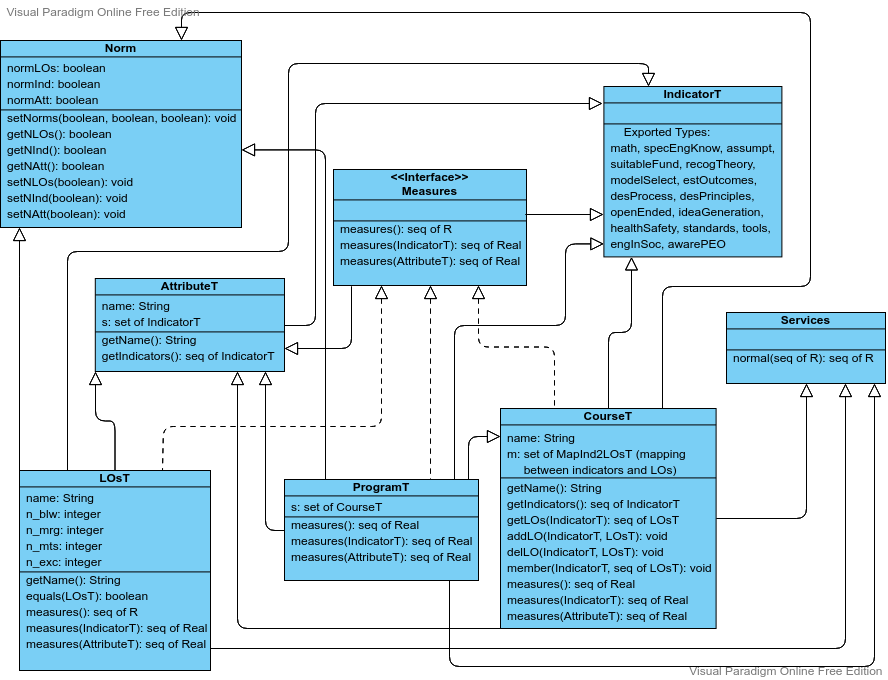
\includegraphics[width=1\textwidth]{A3-UML.png}
\newpage
Q2: Draw a control flow graph for the convex hull algorithm.  The graph should follow the approach used by the Ghezzi et al.\ textbook.\\


\end {document}